\documentclass[11pt]{article}
\usepackage{acl2014}
\usepackage{times}
\usepackage{url}
\usepackage{latexsym}


%pseudocode:
\usepackage{algorithm}
\usepackage{algpseudocode} 

%figures:
\usepackage{tikz}
\usetikzlibrary{trees,positioning,backgrounds}
\usepackage{tikz-qtree}
\usepackage{subcaption}

%references and keeping floats in place
\usepackage{hyperref}
\usepackage[section]{placeins}

\usepackage{amsmath} 

\title{A comparison of \ddop~and \dops}
\author{Benno Kruit\\10576223\\benno.kruit@student.uva.nl\And
Sara Veldhoen\\10545298\\sara.veldhoen@student.uva.nl}
\date{}


\begin{document}
%NB: gebruik \dops{} of \dops~ om netjes een whitespace erachter te krijgen in lopende tekst
\newcommand{\dops}[0]{DOP$ ^*$}
\newcommand{\ddop}[0]{Double-DOP}

\maketitle

\begin{abstract}
This paper investigates two existing estimators in the Data Oriented Parsing approach to natural language syntax. We assess the theoretical and practical differences between these estimators by comparing the grammars they derive.
\end{abstract}


\section{Introduction}
%Introduction to the paper
%General introduction to the DOP framework, terminology 
%NB: introduce term 'fragment' for usage throughout this document



%Je hebt de introductie en terminologie helemaal uit elkaar getrokken. Wat op zich wel helder is, maar niet zo compact.. Aangezien we maar 9 pagina's mogen schrijven kunnen we dat denk ik beter samenvoegen.


A common approach to natural language syntax, is to view the structure of sentences as constituent trees. Such trees can be described by a \emph{Context Free Grammars} (CFGs),  such that all trees are built up from  rules that each describe the production (children nodes) of a single node (parent) in the tree. When building an empirical model of observed parse trees, these rules are extended with probabilities to form a \emph{probabilistic CFG} (PCFG). This gives the trees that are `generated' by these rules their own probability, which makes it a statistical model of a distribution over natural language syntax.

The simple rules of a CFG cannot describe all linguistic phenomena, such as long distance dependencies. Grammars can be enriched by Markovisation, to include deeper levels in the tree. 


\subsection{DOP}
\emph{Data-Oriented Parsing} (DOP), as first introduced in\cite{scha1990}, takes a different approach. It models the language with a Probabilistic Tree Substitution Grammar (PTSG). 
The trees in the treebank are taken apart, which results in \emph{fragments} of arbitrary depth. A fragment is a connected subgraph of a tree such that it corresponds to context-free productions in that tree, i.e. each node must have either have children with the same labels as in the original tree, or no children at all. Note that a level-one fragment corresponds to a CFG rule. Its \emph{symbolic grammar} refers to the set of fragments (that receive a non-zero weight) in a grammar. 

Fragments can be combined in a \emph{derivation} to build syntactic structures. A step in a derivation is a composition, denoted by the symbol $\circ$. We follow the convention to only allow left-most derivations. This means that the left-most non-terminal node in a fragment $f_1$ must correspond to the root node of $f_2$ in order to derive $f_3=f_1\circ f_2$

For each fragment, the probability is estimated by counting how often it occurs in the treebank, compared to others with the same root. The probability of a derivation is the product of the probability of the fragments. Note that a single tree can be the result of different derivations. Therefore probability of a tree is the sum of the probabilities of all its derivations.

\subsection{Theoretical issues}
It has been argued that DOP (in its original formulation) is biased and inconsistent \cite{johnson2002}, both assumed to be bad properties of an estimator in general. As we will see, bias is not necessarily a bad thing. In fact, \cite{zollmann2005} proves that any non-overfitting estimator is biased. Furthermore, he shows that it is possible to define a DOP-estimator that is consistent.


\subsection{Practical issues}
In its original formulation, DOP takes the trees apart in all possible ways. The number of fragments is exponential in the length of the sentences, thus the size of the symbolic grammar would be far too huge to be computationally feasible. 
Different approaches have been taken to reduce the symbolic grammar, e.g. by sampling or by applying a smart algorithm. This appears to be far from trivial.


\subsection{Outlook}
Section~\ref{sec:Statistics} elaborates the notions of consistency and bias and their relation to overfitting.
In section~\ref{sec:Existing}, we outline two approaches that tackle the reduction of the symbolic grammars: \ddop{} and \dops{}. This report focuses on a comparison of these approaches. Theoretically, they differ in that \dops{}, unlike \ddop{}, has been proven to be consistent \cite{zollmann2005}. We investigate the differences between the grammars produced by \ddop{} \dops{}. The algorithms can be decomposed into two parts. We also analyze the impact of the partial choices by mutually using these parts.

Section~\ref{sec:Comparison} offers a detailed comparison of the two methods as well as a description of the experiments we conduct. In section~\ref{sec:Results}, we present our findings and provide an analysis. 



\section{Statistics: Consistency and Bias}\label{sec:Statistics}

% TODO: Cite Dop*!

% Distribution, sampling, estimation, corpus.
% /Linguistic studies of syntax mostly concern \emph{competence} models, which describe the structures that appear in a language. In contrast, a \emph{performance} model of language is an estimate of the probability of observing a parse tree in language use. It treats language as a statistical distribution over syntactic structures.
To be able to reliably parse sentences, it's most effective to model language as a statistical distribution over syntactic structures. This means we'll have to estimate the probability of observing a parse tree in language use. 

Let $\Omega$ be the set of all possible parse trees. The distribution $P_\Omega: \Omega\rightarrow [0,1]$ then describes a language, where $P_\Omega(t)$ is the probability of observing a tree $t \in \Omega$. Using a sample of parse trees from the language, an \emph{estimator} $\textsc{est}$ builds a statistical model. A parser then uses that statistical model to predict the correct parse tree of sentences.
A sample $X \in \Omega^n$ from the language is called a \emph{corpus} or \emph{treebank} of size $n$, which makes $\textsc{est}(X)$ an estimator trained on a sample. If $\mathcal{M}$ is the set of probability distributions over $\Omega$, then $P_\Omega \in \mathcal{M}$ and $\textsc{est}(X) \in \mathcal{M}$.

% Expectation given a distribution, Loss, risk, mean squared difference, error.
In theory, an estimator should make exactly the right estimations of probabilities if it's given an infinite amount of data. That is to say, it should \emph{converge} to the true distribution. If an estimator converges in the limit, that estimator is \emph{consistent} \cite{zollmann2005}.
However, given a finite amount of data, the estimator will probably not generate the correct distribution. The distance between the true distribution $P^*$ and an estimate $P$ is called the \emph{loss} of that estimate. The loss can be defined in different ways, but the most popular is the \emph{mean squared difference}:

$$ \mathcal{L}(P, P^*) =  \sum_{t \in \Omega} P^*(t) (P^*(t)-P(t))^2$$

From a true distribution, it's possible to calculate the expected loss of an estimator trained on a treebank of a certain size. This is the \emph{risk} or \emph{error} of that estimator given a sample size and a distribution. 
% When sampling $X$ of size $n$ from $P^*$,
% $$ error(\textsc{est}, P^*) = \mathbf{E}[\mathcal{L}(\textsc{est}(X), P^*)]$$
When the sample size approaches the limit, the error of an estimator should diminish. With these definitions, it is possible to define estimator consistency when sampling $X \in \Omega^n$ from $P_\Omega$:

$$\lim_{n \to \infty} \mathbf{E}[\mathcal{L}(\textsc{est}(X), P_\Omega)] = 0 $$

% Estimators: RF, EWE?, MLE?

In its original formulation, DOP was defined using a \emph{relative frequency estimate}, by counting how often it occurs in the treebank compared to others with the same root. However, it has been shown \cite{johnson2002} that in this case, the RF estimator is inconsistent.

% Bias
Another property of an estimator is its \emph{bias}, which is defined as the difference between the true probability distribution and the expected estimate for a language. If a language exists for which this difference is nonzero, the estimator is biased in general. We will see that bias is a desirable property for the DOP model.
% It has been proven \cite{zollman2005} that any unbiased DOP estimator will overfit a treebank by assigning zero-probabilites to trees outside the corpus.
% To prevent overfitting, it is therefore necessary to introduce a bias that assigns a non-zero probability to unseen trees.
% By maximizing the probability of a corpus different from the one from which the fragments are extracted, we will see that it is possible to minimize overfitting.

% Add this to 3.2.2 ??



\section{Existing Models: Double-DOP and DOP$^*$}\label{sec:Existing}
%A description and comparison of Double-DOP and DOP*

%Iets met Goodman? Die behoudt alleen kleine stukjes en speciale regels, maar daardoor geen expliciete representatie van 'productive units' (Sangati, einde van sectie 2)

In this section, we outline two approaches to constrain the extraction of fragments: \ddop{} and \dops{}. Furthermore, we discuss the similarities and dissimilarities for these two approaches. 

\subsection{\ddop}
In the following, we discuss \ddop{} as it was presented in \cite{sangati2011}. In this model, no unique fragments are extracted from the dataset: if a construction occurs in one tree only, it is probably not representative for the language. This is carried out by a dynamic algorithm using tree-kernels. It iterates over pairs of trees in the treebank, looking for fragments they have in common. In fact, only the largest shared fragment is stored. 

The symbolic grammar that is the output of this algorithmis not guaranteed to derive each tree in the training corpus. Therefore all one-level fragments, consitutuing the set of PCFG-productions, are also added.

The \ddop{} model describes an extraction method for determining the symbolic grammar. However, it was also implemented with different estimators. The estimation is done in a second pass over the treebank, gathering frequency counts for the fragments in the gramar. 

The best maximizing objective appears to be MCP (max consituent parse), which maximizes a weighted average of expected labeled recall and precision. The latter cannot be maximized directly, but is approximated by minimizing the mistake rate. 
Parameter $\lambda$ that rules the linear interpolation was empirically found to be optimal at 1.15. Efficient calculation of MPC is possible with dynamic programming, but it can also be approximated with a list of $k$-best derivations.

In addition, empirical results show that the relative frequency estimate outperforms the other estimates tested, i.e. Equal Weights Estimate (first adjust counts proportional to the size of the symbolic grammar, this value proportional to fragments with the same root), and Maximum Likelihood (optimizing to maximum likelihood for the training data with an Inside-Outside algorithm). 
%NB in contrast to earlier findings
%NB: unknown words approach: rare words, frequency <5, get a general tag based on morphological features

\subsection{\dops}
In \dops{} \cite{zollmann2005}, a rather different approach is taken called held-out estimation. The treebank is split in two parts, the extraction corpus ($EC$) and a held-out corpus ($HC$). An initial set of fragments is extracted from the $EC$, containing all the fragments from its trees. The weights are then determined so as to to maximize the likelihood of $HC$, under the assumption that this is equivalent to maximizing the joint probability of the \emph{shortest derivations} of the trees in $HC$. All fragments that do not occur in such a derivation are removed from the symbolic grammar. 
Note that some trees in $HC$ may not be derivable at all. Furthermore, a tree could have several shortest derivations. 

\paragraph{Consistency and bias}
\dops{} was claimed to be the first consistent (non-trivial) DOP-estimator, \cite{zollmann2005} provides a consistency proof. On the other hand \dops{} is  biased, but Zollmann shows how bias actually arises from generalization: no non-overfitting DOP estimator could be unbiased. Bias is therefore not prohibited but on the contrary a desirable property of an estimator.

In \cite{zuidema2006} it is argued that there is a problem with the consistency proof given for \dops{}, as well as the non-consistency proof for other DOP-estimators by \cite{johnson2002}. Zuidema points out that these proofs use a frequency-distribution test, whereas for DOP a weight-distribution test would be more appropriate. 
%Wat hiermee?
























\section{Comparison} \label{sec:Comparison}
%The theoretical properties of \dops{} and \ddop{} differ:  
\dops{} and \ddop{} differ both in the set of fragments they extract and their estimation of the weights. To investigate the exact differences, we will view both steps separately.

%Note that the \dops{} extraction needs another decision: in many cases, there are several shortest derivations possible. From now on, we add all fragments that occur in one of these shortest derivations to the symbolic grammar. Of course we need to adjust the weights (e.g. divide the frequency counts by the number of shortest derivations) so that no full tree gets a higher impact on the PTSG. We will keep to the original formulation of \dops{} in case no derivation is possible, i.e. not including any fragments for this tree.

\paragraph{Extraction}
\ddop{} uses a tree kernel approach to find the maximal overlapping fragments of pairs of trees, which are added to the symbolic grammar. We will call this the \emph{maximal-overlap} method. \dops{} iteratively finds the shortest derivation of one tree given all the fragments of a set of trees, hereafter the \emph{shortest-derivation} method. 

It is easy to see that the \emph{shortest-derivation} extraction in itself does not depend on the corpus split: we can also find the shortest possible derivation using fragments from all the other trees. Likewise \ddop{} could be implemented using a split, comparing all trees in the $HC$ to all trees in the $EC$.
We will refer to these methods as \emph{one vs. rest} and \emph{split} estimation.

%Whether the corpus is split in two does only influence the size of the symbolic grammar and

%Therefore, w
%We will implement both extraction methods in a 1 vs the rest manner. In this way, we can analyse how the resulting symbolic grammars differ. The analysis will comprise the size of the resulting symbolic grammar and the relative number of fragments of certain depth. Furthermore, we might be able to find interesting patterns by manually looking at the fragments that were extracted by one of the systems only.

\paragraph{Estimation}

Both approaches use the relative frequencies of the fragments for the weights:
\begin{align}p(f)=\frac{count(f)}{\sum_{f'\in F_{root}(f)} count(f')}\end{align} 
However, in the \ddop{} case these values refer to exact counts of the fragments in the treebank, whereas in \dops{} they refer to occurrence of fragments in shortest derivations.


\ddop{} determines the weights of the fragments in the symbolic grammar in a separate run over the treebank, to obtain exact counts. We use the relative frequency estimate to assign weights to the fragments. \dops{} on the other hand counts the occurrence in shortest derivations of the fragments, and normalizes relative to counts of fragments with the same root.

To maximize coverage of the grammar, both \ddop{} and \dops{} apply smoothing that slightly alters the weights. Next to extracting maximally overlapping fragments, \ddop{} extracts all CFG rules and estimates their weight. \dops{} is smoothed by calculating the weight of the unparsed sentences, and distributes this over the CFG rules.

 %Furthermore, infrequent words are replaced by a lexical description.

%HIER



\paragraph{Example}
\FloatBarrier
This example clarifies how the grammars that result from \ddop{} and \dops{} can actually differ. Recall our toy treebank from figure \ref{f:treebank} and the fragments in figure \ref{f:fragments}. 
Applying the maximal overlap extraction and shortest derivation extraction in a 1 vs the rest manner to this treebank, yields the weights in table \ref{t:weights}.

Note the remarkable differences in the weight distributions. For example, $f_1$ gets a weight of 0.5 in the maximal overlap approach, and zero in the shortest derivation case. Of course, the sparsity of the data contributes much to these extreme variations. However, the observed differences encourage us to investigate these two approaches into more depth.



\begin{table}[h!]
\center
\begin{tabular}{c|p{.10\textwidth}c|p{.08\textwidth}c|}
&Maximal overlap&weight&Shortest deriv.\footnotemark&weight\\\hline
f1&(t1,t3),(t2,t4)&4/12&-&0\\
f2&(t1,t2)&2/12&1b, 2a&1/4\\
f3&(t2,t3)&2/12&2b, 3b&1/4\\
f4&(t3,t4)&2/12&3a, 4b&1/4\\
f5&(t1,t4)&2/12&1a, 4a&1/4\\
f6&(t1,t3),(t1,t4), (t2,t3),(t2,t4)&4/6&1a, 2b&1/2\\
f7&-&0&3b, 4a&1/2\\
f8&CFG rule&2/6&-&0\\
f9&(t2,t3),(t2,t4), (t3,t4)&4/6&2a, 3a&1/2\\
f10&-&0&1b, 4b&1/2\\
f11&CFG rule&2/6&-&0\\
f12&CFG rule&2/2&-&0\\
f13&CFG rule&2/2&-&0\\
\end{tabular}

\caption{The weights assignment according to both methods in a one vs. the rest manner}
\label{t:weights}
\end{table}
\footnotetext{For this dataset, two shortest derivations exist for each tree. We refer to them with the following variables: 1a = f5, f6; 1b = f2, f10; 2a = f2, f8; 2b = f3, f6; 3a = f4, f8; 3b = f3, f7; 4a = f5, f7; 4b = f4, f9}





\subsection{Experiments}
%Description of our implementation, how does it resemble Double-DOP and DOP*? What are the differences? What are the theoretical capabilities? 





We compare the maximal overlap and shortest derivation extraction by using either a split or the whole set of trees for both estimators. We will plot the fragments according to the weights assigned by the estimators, such that the differences can stand out. In the same way, we compare the split and one vs. the rest estimation for the same estimator.

Furthermore, we can compare the grammars by having them parse a test set and determine their performance, e.g. the F1-score for correctly predicted parses.

\paragraph{Data}
We use the \emph{Wall Street Journal}~(WSJ) section of the Penn Treebank for our experiments. \dops{} has only been applied to the Dutch OVIS corpus in \cite{zollmann2005}, which contains relatively small and (therefore) easy sentences. Therefore we are curious about its performance on the WSJ.

The corpus was preprocessed by removing functions and binarizing the trees by Markovization (h=1, v=1). 

\paragraph{Algorithm}
First of all, we find the maximally overlapping fragments of all trees in the corpus, which corresponds to the \ddop{} approach.
Then, we randomly split the corpus ten times in two equally-sized parts, called $EC$ and $HC$. For each split, build a DOP-reduction grammar from $EC$ and use it to find the shortest derivations of the trees in $HC$, which corresponds to \dops{}. Additionally, we find the maximally overlapping fragments and estimate their weights from the $EC$. We'll call this \emph{Split Double-DOP}.

The results for the different splits were interpolated and the resulting grammars were smoothed as described above. For finding the weight of unparsable sentences in the \dops{} estimation, we needed to find the trees that had not been derived in any split. This was done by comparing each set of underived trees with the $HC$ sets of every split.

Estimation and parsing were done with the {\tt disco-dop} framework \ref{cranenburg?}.

\paragraph{Parsing}
The input for the parser consisted of sentences of word and POS tag pairs. The parser matches fragments to the whole pair when the word is known, but only uses the POS tag when the word is unknown.


% Estimating all grammars took 45 hours on 16 CPU cores.

\paragraph{Questions}
Comparing \dops{} and \ddop{}: Which estimator gives more weight to large fragments? Is this related to consistency?

Comparing \ddop{} and Split Double-DOP: What influence does a split have on performance and size of a grammar? How do the fragment weight distributions differ?

Comparing Split Double-DOP and \dops{}: Assuming that a larger weight in \dops{} corresponds to `usefulness' in parsing, what determines whether a fragment is useful?


%
%
%\paragraph{Extraction}
%Algorithm \ref{a:dops2} performs shortest-derivation extraction (as in \dops{}) in an efficient way, resembling the tree kernel approach in the iterative comparison of one tree with others. Namely, we iterate over the trees in $HC$ (lines 2-8): create a list $F$ of all of its fragments that occur in the rest of the treebank (line 3) and increment the count of the fragments in $F$ that occur in the shortest derivation(s). In this way, we do not need to store all fragments in $EC$ as in the initial step of the original \dops{} algorithm. 
%
%Algorithm \ref{a:ddop1} performs the maximal-overlap extraction (as in \ddop{}). For the comparison of trees to find the maximal overlap (line 4), the tree kernel approach from \cite{sangati2011} is used. 
%
%\begin{algorithm}
%{\bf Data}: a treebank $TB$\\
%{\bf Result}: a map of tree fragments and corresponding counts in shortest derivations\\
%\begin{algorithmic}[1]
%\State{Initialize $M$, a map from fragments to counts, empty}
%\For {$t\in TB$}
%	\State $F \gets Frag(t)\cap \bigcup\limits_{t'\in TB/\{t\}} frag(t')$
%	\State{$D\gets$ the shortest derivation(s) of $t$ using fragments in $F$}		
%	\For{$f\in D$}
%		\State add $f$ to $M$ {\bf if} $f\not\in M$
%		\State $M[f]\gets M[f]+1$ \Comment{Anticipating the estimation step}
%	\EndFor
%\EndFor
%%\For{$n \in V_N$}
%%	\State{Add the counts of all fragments rooted at $n$}
%%	\State{Normalize the weights of these fragments}
%%\EndFor	
%\end{algorithmic}
%\caption{Shortest derivation extraction in a one vs the rest manner}
%\label{a:dops2}
%\end{algorithm}
%
%
%\begin{algorithm}
%{\bf Data}: a treebank $TB$\\
%{\bf Result}: a set of tree fragments\\
%\begin{algorithmic}[1]
%\State{Initialize $M$, a map from fragments to weights, empty}
%\For{$t\in TB$}
%	\For{$t'\in TB/\{t\}$}
%		\State $f\gets$ maximal overlapping fragment(s) of $t$ and $t'$
%		\State add $f$ to $M$ {\bf if} $f\not\in M$
%	\EndFor
%\EndFor
%\end{algorithmic}
%
%
%
%\caption{Maximal overlap extraction in a one vs the rest manner}
%\label{a:ddop1}
%\end{algorithm}
%
%\paragraph{Estimation}
%Now for estimation, we use the output of the extraction algorithm. In the case of shortest-derivation extraction (algorithm \ref{a:dops2}), we only need to normalize the counts in $M$ to their relative frequency as compared to fragments that have the same root. In the case of maximal-overlap extraction (algorithm \ref{a:ddop1}), we need to iterate over the dataset once more to count the occurences of the fragments in the output and then compute their relative frequencies.
%
%%In \ddop, we would iterate over pairs of trees. With treebank size $n$, that would require $n!$%NEEN klopt niet! comparisons. In our proposed algorithm, we need to iterate over each combination of a tree in $HC$ with (worst case\footnote{The condition in line $5$ avoids unnecessary search for fragments. We might be able to pose a smarter constraint here, such that we only continue if we can possibly find fragments that lead to a shorter derivation}) all trees in $EC$. This requires $n/2 \times n/2$ comparisons. Furthermore, we immediately store the counts, so we don't need to iterate over the data again to assess the weights. We do however need to normalize the weights, such that the sum of weights of all fragment sharing the same root equals 1.




%In words: Iterate over the trees in $HC$ (lines 2-17): create a list $F$ of all of its fragments that occur in $EC$ (lines 3-12). This procedure resembles the treekernels from \ddop. Create the shortest derivation $D$ from fragments in $F$ (NB: this is not always possible, in which case $D=\emptyset$). Increment the counts of these fragments in the map $M$

%\begin{algorithm}[H]
%{\bf Data}: non-overlapping treebanks $EC$ and $HC$\\
%{\bf Result}: a PTSG, i.e. a map of tree fragments and corresponding weights\\
%\begin{algorithmic}[1]
%\State{Initialize $M$, a map from fragments to weights, empty}
%\For {$t_H\in HC$}
%%	\State $Q\gets frag(t_H)$
%%	\State $F \gets \emptyset$
%%	\While{$Q$ not empty}% or a smarter constraint
%%		\For{$t_E \in EC$}
%%			\For{$f \in Q\cap frag(t_E)$}
%%				\State $Q\gets Q/\{f\}$	
%%				\State $F\gets F\cup\{f\}$	
%%			\EndFor
%%		\EndFor
%%	\EndWhile
%	\State $F \gets Frag(t_H)\cap \bigcup\limits_{t_E\in EC} frag(t_E)$
%	\State{$D\gets$ the shortest derivation of $t_H$ using fragments in $F$}		
%	\For{$f\in D$}
%		\State add $f$ to $M$ {\bf if} $f\not\in M$
%		\State $M[f]\gets M[f]+1$
%	\EndFor
%\EndFor
%\For{$n \in V_N$}
%	\State{Add the counts of all fragments rooted at $n$}
%	\State{Normalize the weights of these fragments}
%\EndFor	
%\end{algorithmic}
%\caption{\dops{} extraction and estimation}
%\label{a:dops1}
%\end{algorithm}

\section{Results and analysis}\label{sec:Results}
\begin{figure}[h!]
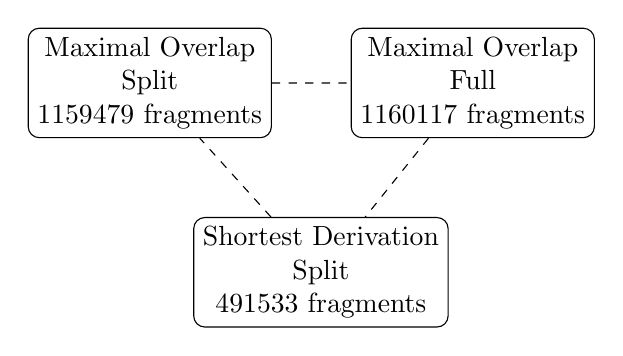
\begin{tikzpicture}[node distance = 1cm]
\node (MOS) [rectangle,rounded corners,draw, align=center]{Maximal Overlap\\ Split\\1159479 fragments};
\node (MOF) [right = of MOS, rectangle,rounded corners,draw, align=center]{Maximal Overlap\\ Full\\1160117 fragments};
\node (SDS) [below right= 1 cm and -1 cm of MOS, rectangle,rounded corners,draw, align=center]{Shortest Derivation\\ Split\\491533 fragments};
\draw[dashed](MOS)--(MOF)--(SDS)--(MOS);
\end{tikzpicture}
\caption{The grammars and their size}
\label{f:grammars}
\end{figure}
%SIZE OF THE GRAMMARs

Figure \ref{f:grammars} summarizes the three grammars we investigate.
%There are three grammars we analyze: maximal overlap extraction with both split and full estimation, and shortest derivation with split estimation.
The split estimation was done by interpolating the estimates produced by ten random (equal) splits.  All grammars have been smoothed with PCFG rules to maximize coverage. In the maximal overlap approach, this is done internally as defined in \ddop{}. In the shortest derivation apporach, we redistribute a proportion $p_{unkn}$ of the probability mass over the PCFG grammar. $p_{unkn}$ was found to be $1.41\times 10^{-3}$ for our dataset.%0.00140590480016

%Iets over tijd?
%	Het koste slechts 45 uur met 2 servers:
%	$ time sh batch.sh wsj-02-21.mrg 39833 1 5
%	$ time sh batch.sh wsj-02-21.mrg 39833 6 10
%	[...]
%	2490344.51user 2819.26system 44:37:59elapsed 1551%CPU (0avgtext+0avgdata23866400maxresident)k
%	32056inputs+1353048outputs (13major+375643658minor)pagefaults 0swaps

\subsection{Parsing performance}

\begin{table*}
\center
%
%\begin{tabular}{l | ccc}
%&Maximal~Overlap&Maximal~Overlap&Shortest~Derivation\\
%&Full& Split&Split\\\hline
%labeled recall&		90,97&	90.14&	84.90\\
%labeled precision&		90.25&	90.10&	84.39\\
%labeled f-measure&		90.61&	90.12&	84.64\\
%exact match&		53.27&	49.53&	39.25\\
%\end{tabular}
%
%\caption{Results for 321 sentences of length$\leq 15$}
%


\begin{tabular}{l | ccc}
&Maximal~Overlap&Maximal~Overlap&Shortest~Derivation\\
& Full& Split&Split\\\hline
labeled recall&		86.17&	85.11&	79.20\\
labeled precision&		86.05&	85.50&	79.32\\
labeled f-measure&		86.11&	85.31&	79.26\\
exact match&		28.32&	25.87&	16.52\\
\end{tabular}

\caption{Results for 1229 sentences of length$\leq 40$}


\label{t:performance}
\end{table*}

Table \ref{t:performance} shows the parsing performance for the three grammars we constructed. Note that the POS-tags were passed to the parser in all cases, so tagging accuracy was 100\% and is omitted from this table. 
Note that we did only one run on a predefined train/ test split.

Both Maximal Overlap grammars perform much better than the Shortest Derivation one, in spite of the latter being consistent. 
This might well be related to the size of the grammars: the Shortest Derivation grammar has less than half the number of fragments the other two grammars have. 

A second explanation might be the smoothing we conducted. Recall that the coverage of the Maximal Overlap approach is catered in a rather natural way, by extending the symbolic grammar with all PCFG rules from the treebank and treating them like the other fragments in the estimation. In the case of Shortest Derivation however, the coverage was a bit more artificial. $p_{unkn}$ was computed over all folds and used to redistribute weights over a classical PCFG constructed from the entire treebank. 


Furthermore, we observe that the performance of Maximal Overlap with Full estimation performs slightly better than the Split estimation. The latter was expected to prevent overfitting, but apparently was not helpful in this case. As the weights of these two grammars do not diverge much, it would be recommended to do several runs (with different splits for train and test set). This was however not feasible for us, given the limited amount of time for this project.


\subsection{Pairwise comparison of the grammars}
In each plot, two grammars are compared to each other. The fragments are presented in a scatter plot, with the weights assigned by the two grammars along the axes. The weights are best visualized on a logarithmic scale. However, it is also informative to see those fragments with value zero. Therefore, the first interval ($[0,10^{-6}]$) is linear, while the rest of the plot is logarithmic. 
The difference between grammars is represented by the distance of the points to the \emph{identity line} $x=y$.
The color corresponds to some feature, e.g. the depth of the fragment. The color mapping is also logarithmic. 

% 1 figuur:
% SDS MOS depth (both split)
% SDS MOF depth (original DDOP en DOP*)
% MOS MOF depth (split vs full)
\begin{figure*}
\center
\begin{subfigure}{0.32\textwidth}
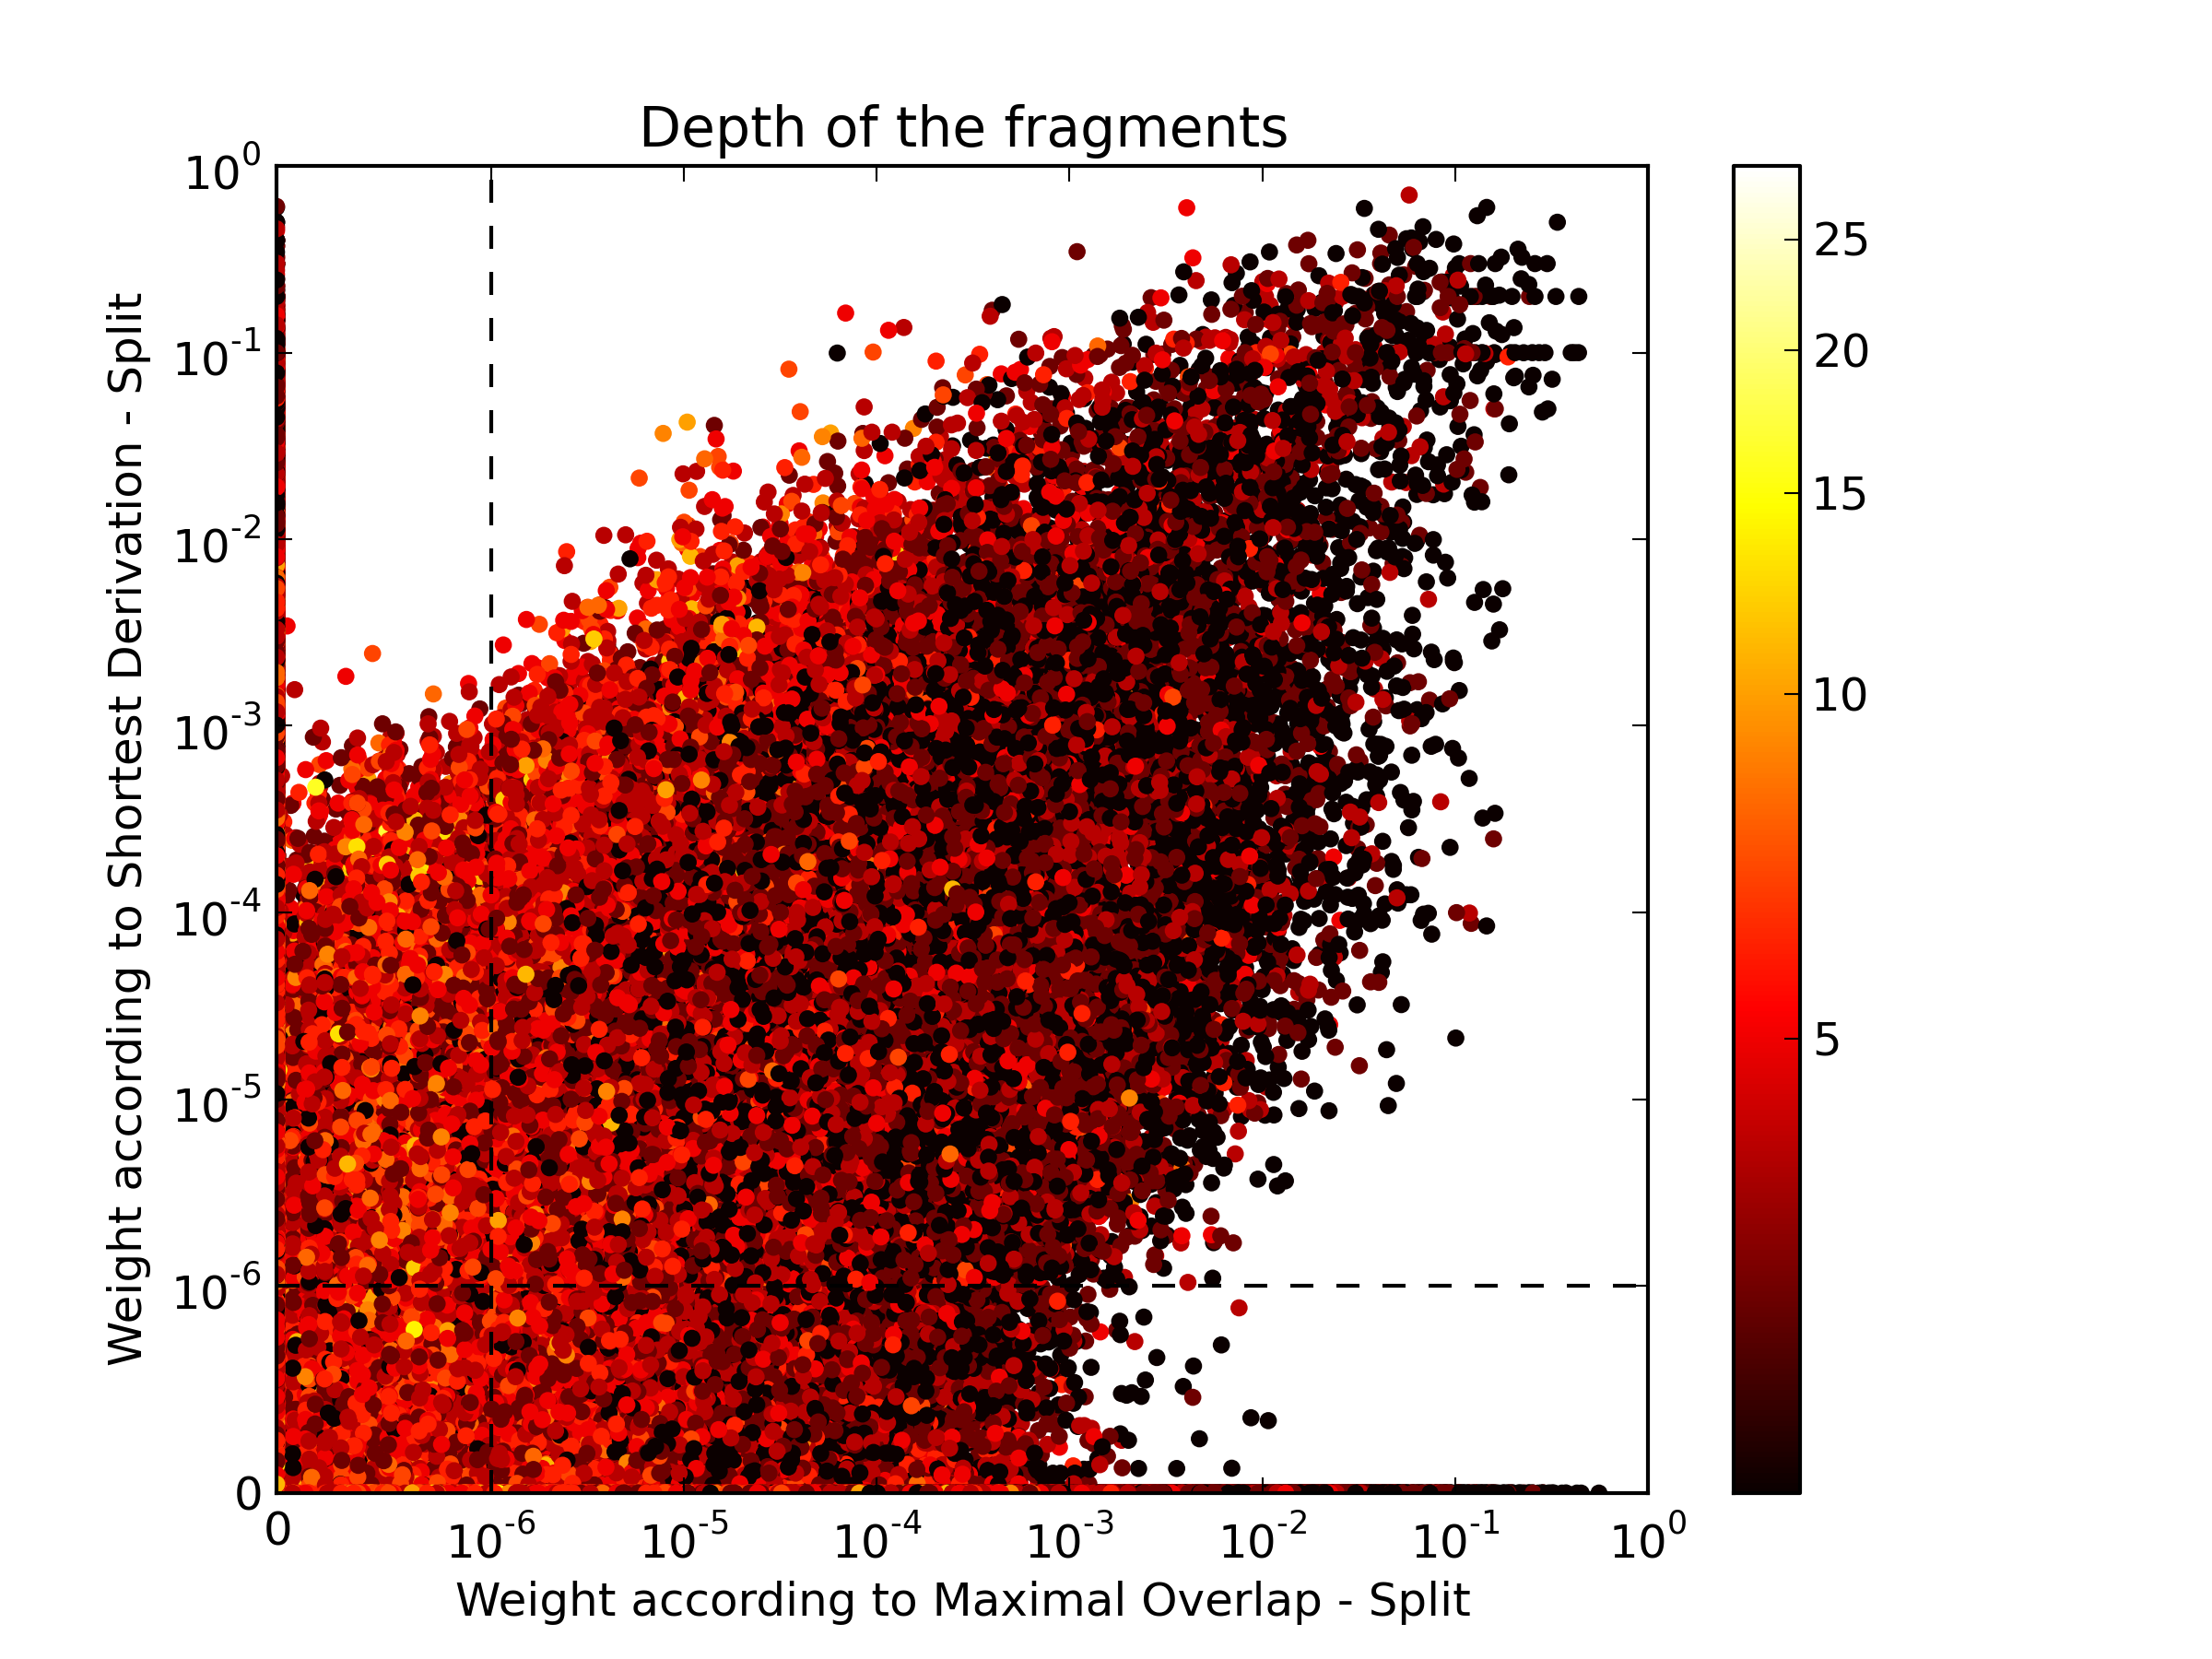
\includegraphics[width=\linewidth,trim=0.5cm 0cm 2.5cm 0.5cm, clip=true]{../data/plots/0.png}
\caption{}
\label{f:SDS-MOS}
\end{subfigure}
\begin{subfigure}{0.32\textwidth}
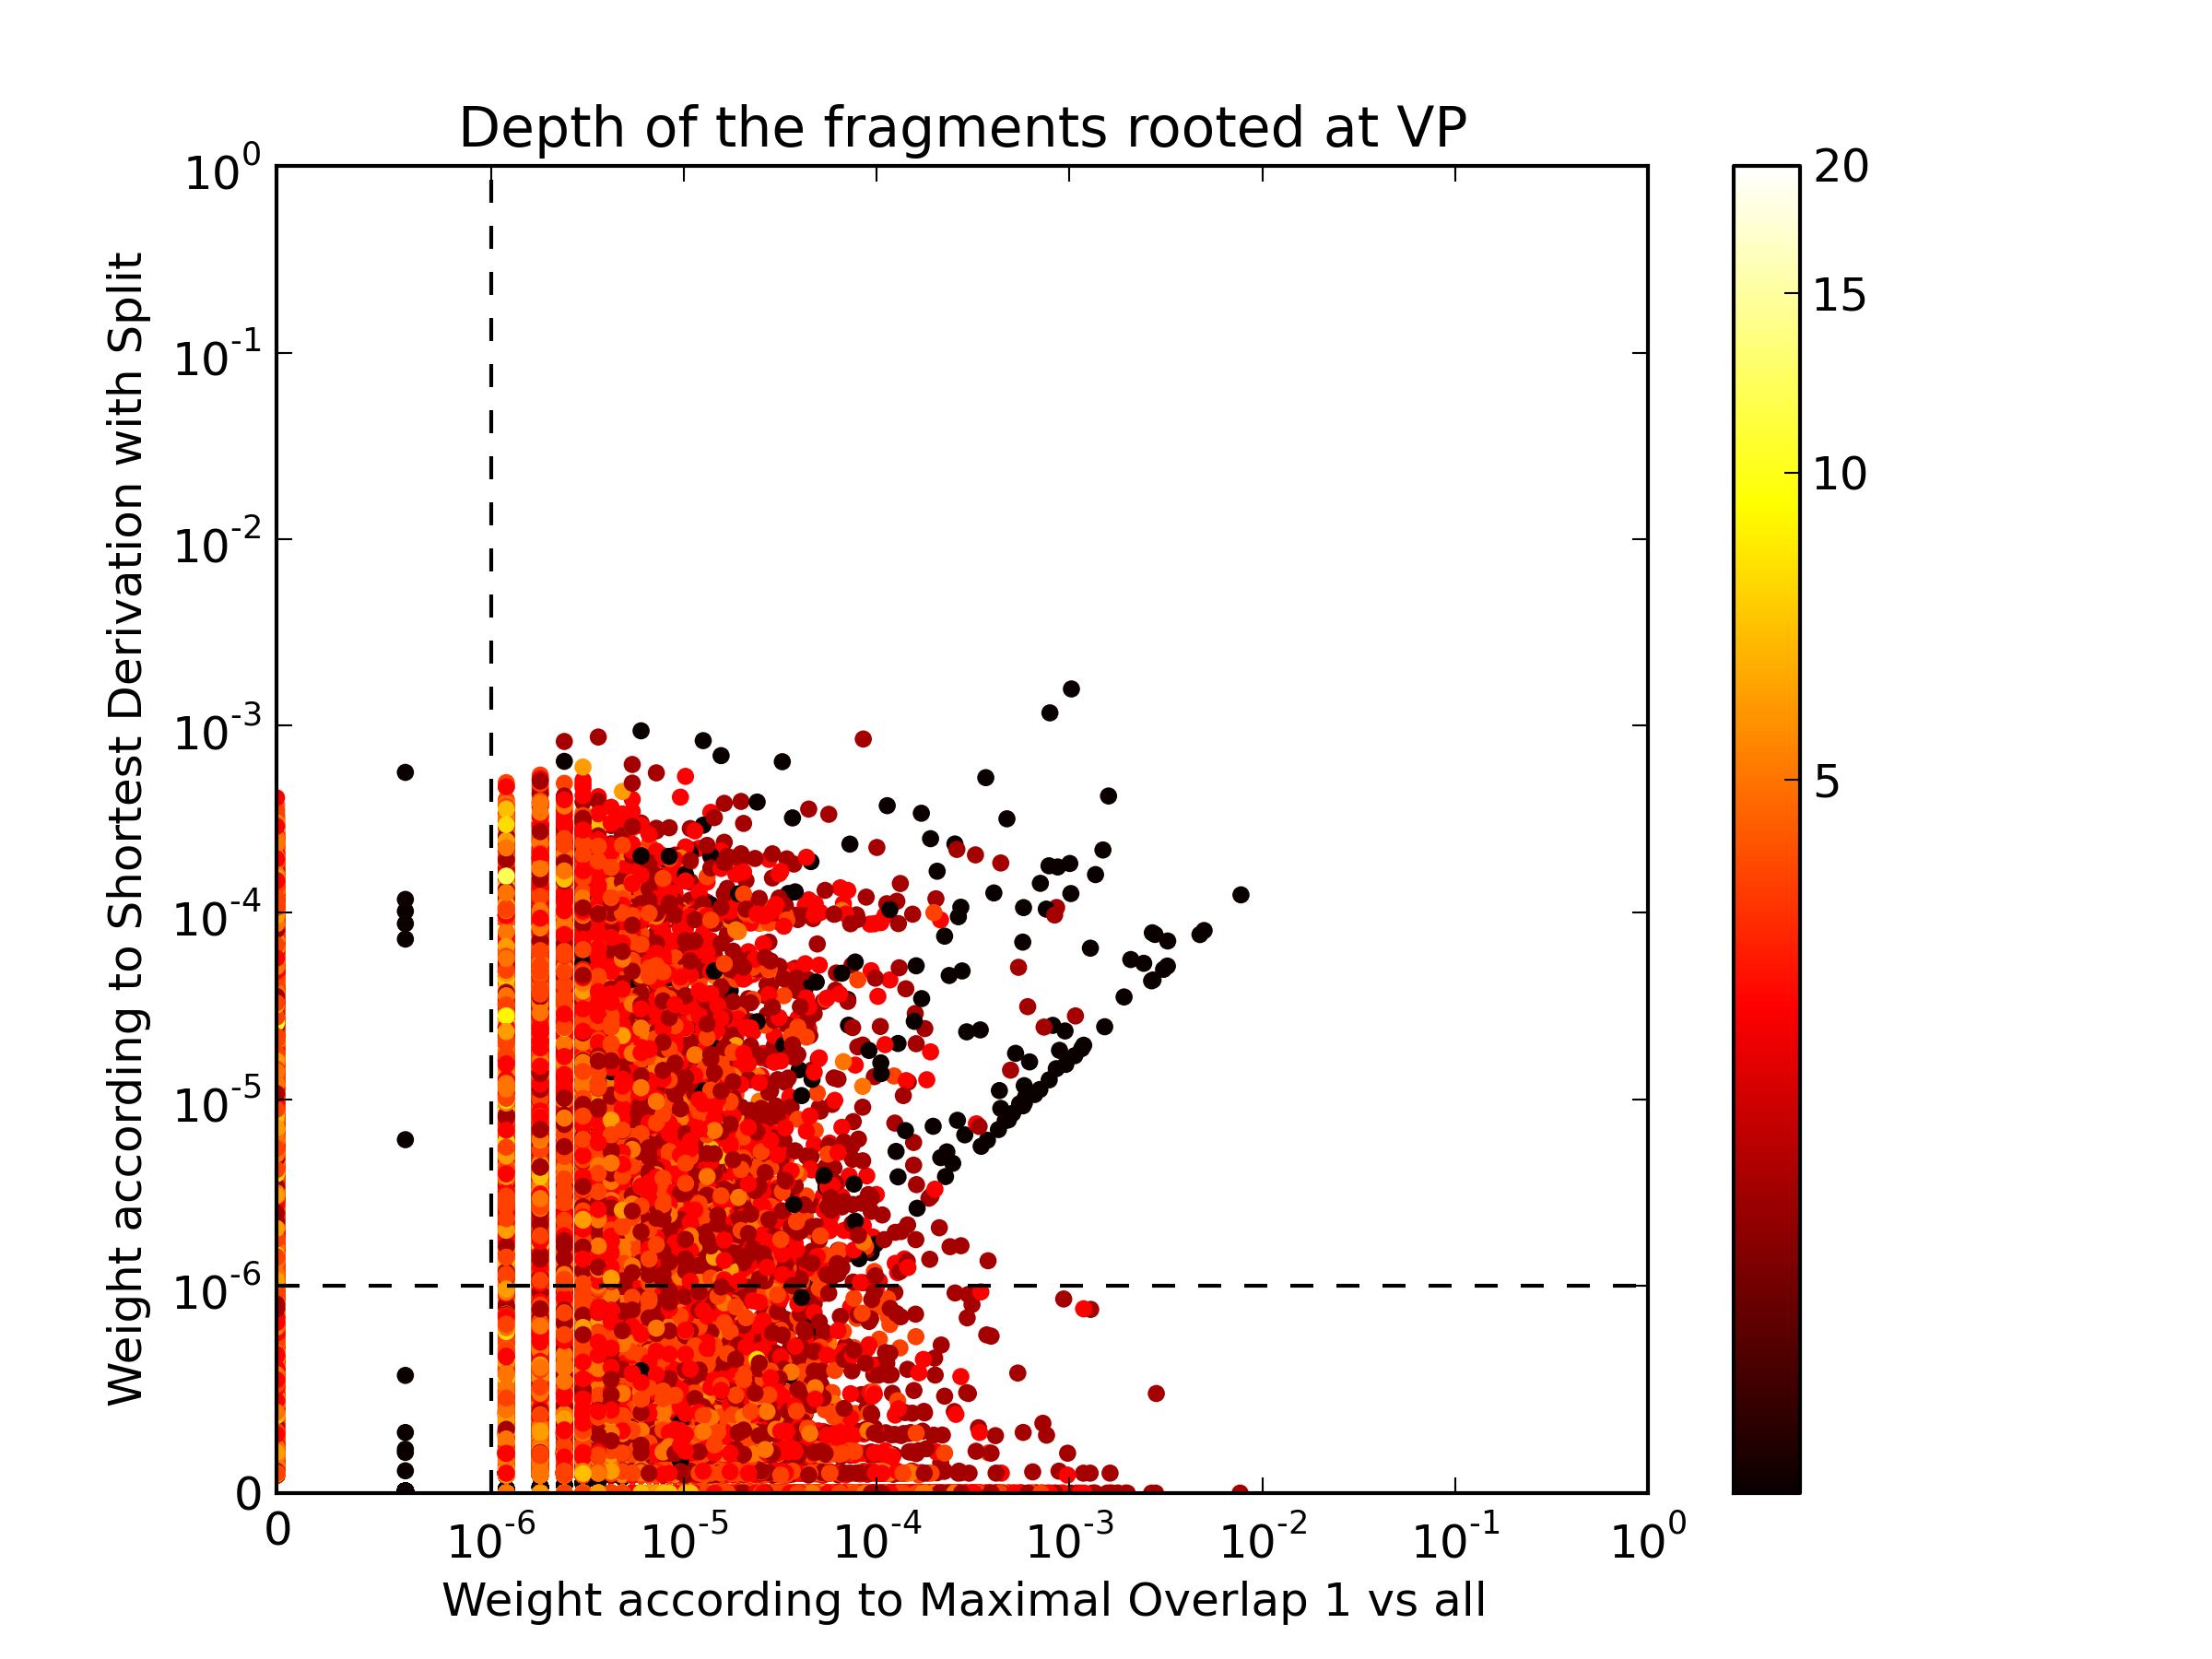
\includegraphics[width=\linewidth,trim=0.5cm 0cm 2.5cm 0.5cm, clip=true]{../data/plots/1.png}
\caption{}
\label{f:SDS-MOF}
\end{subfigure}
\begin{subfigure}{0.32\textwidth}
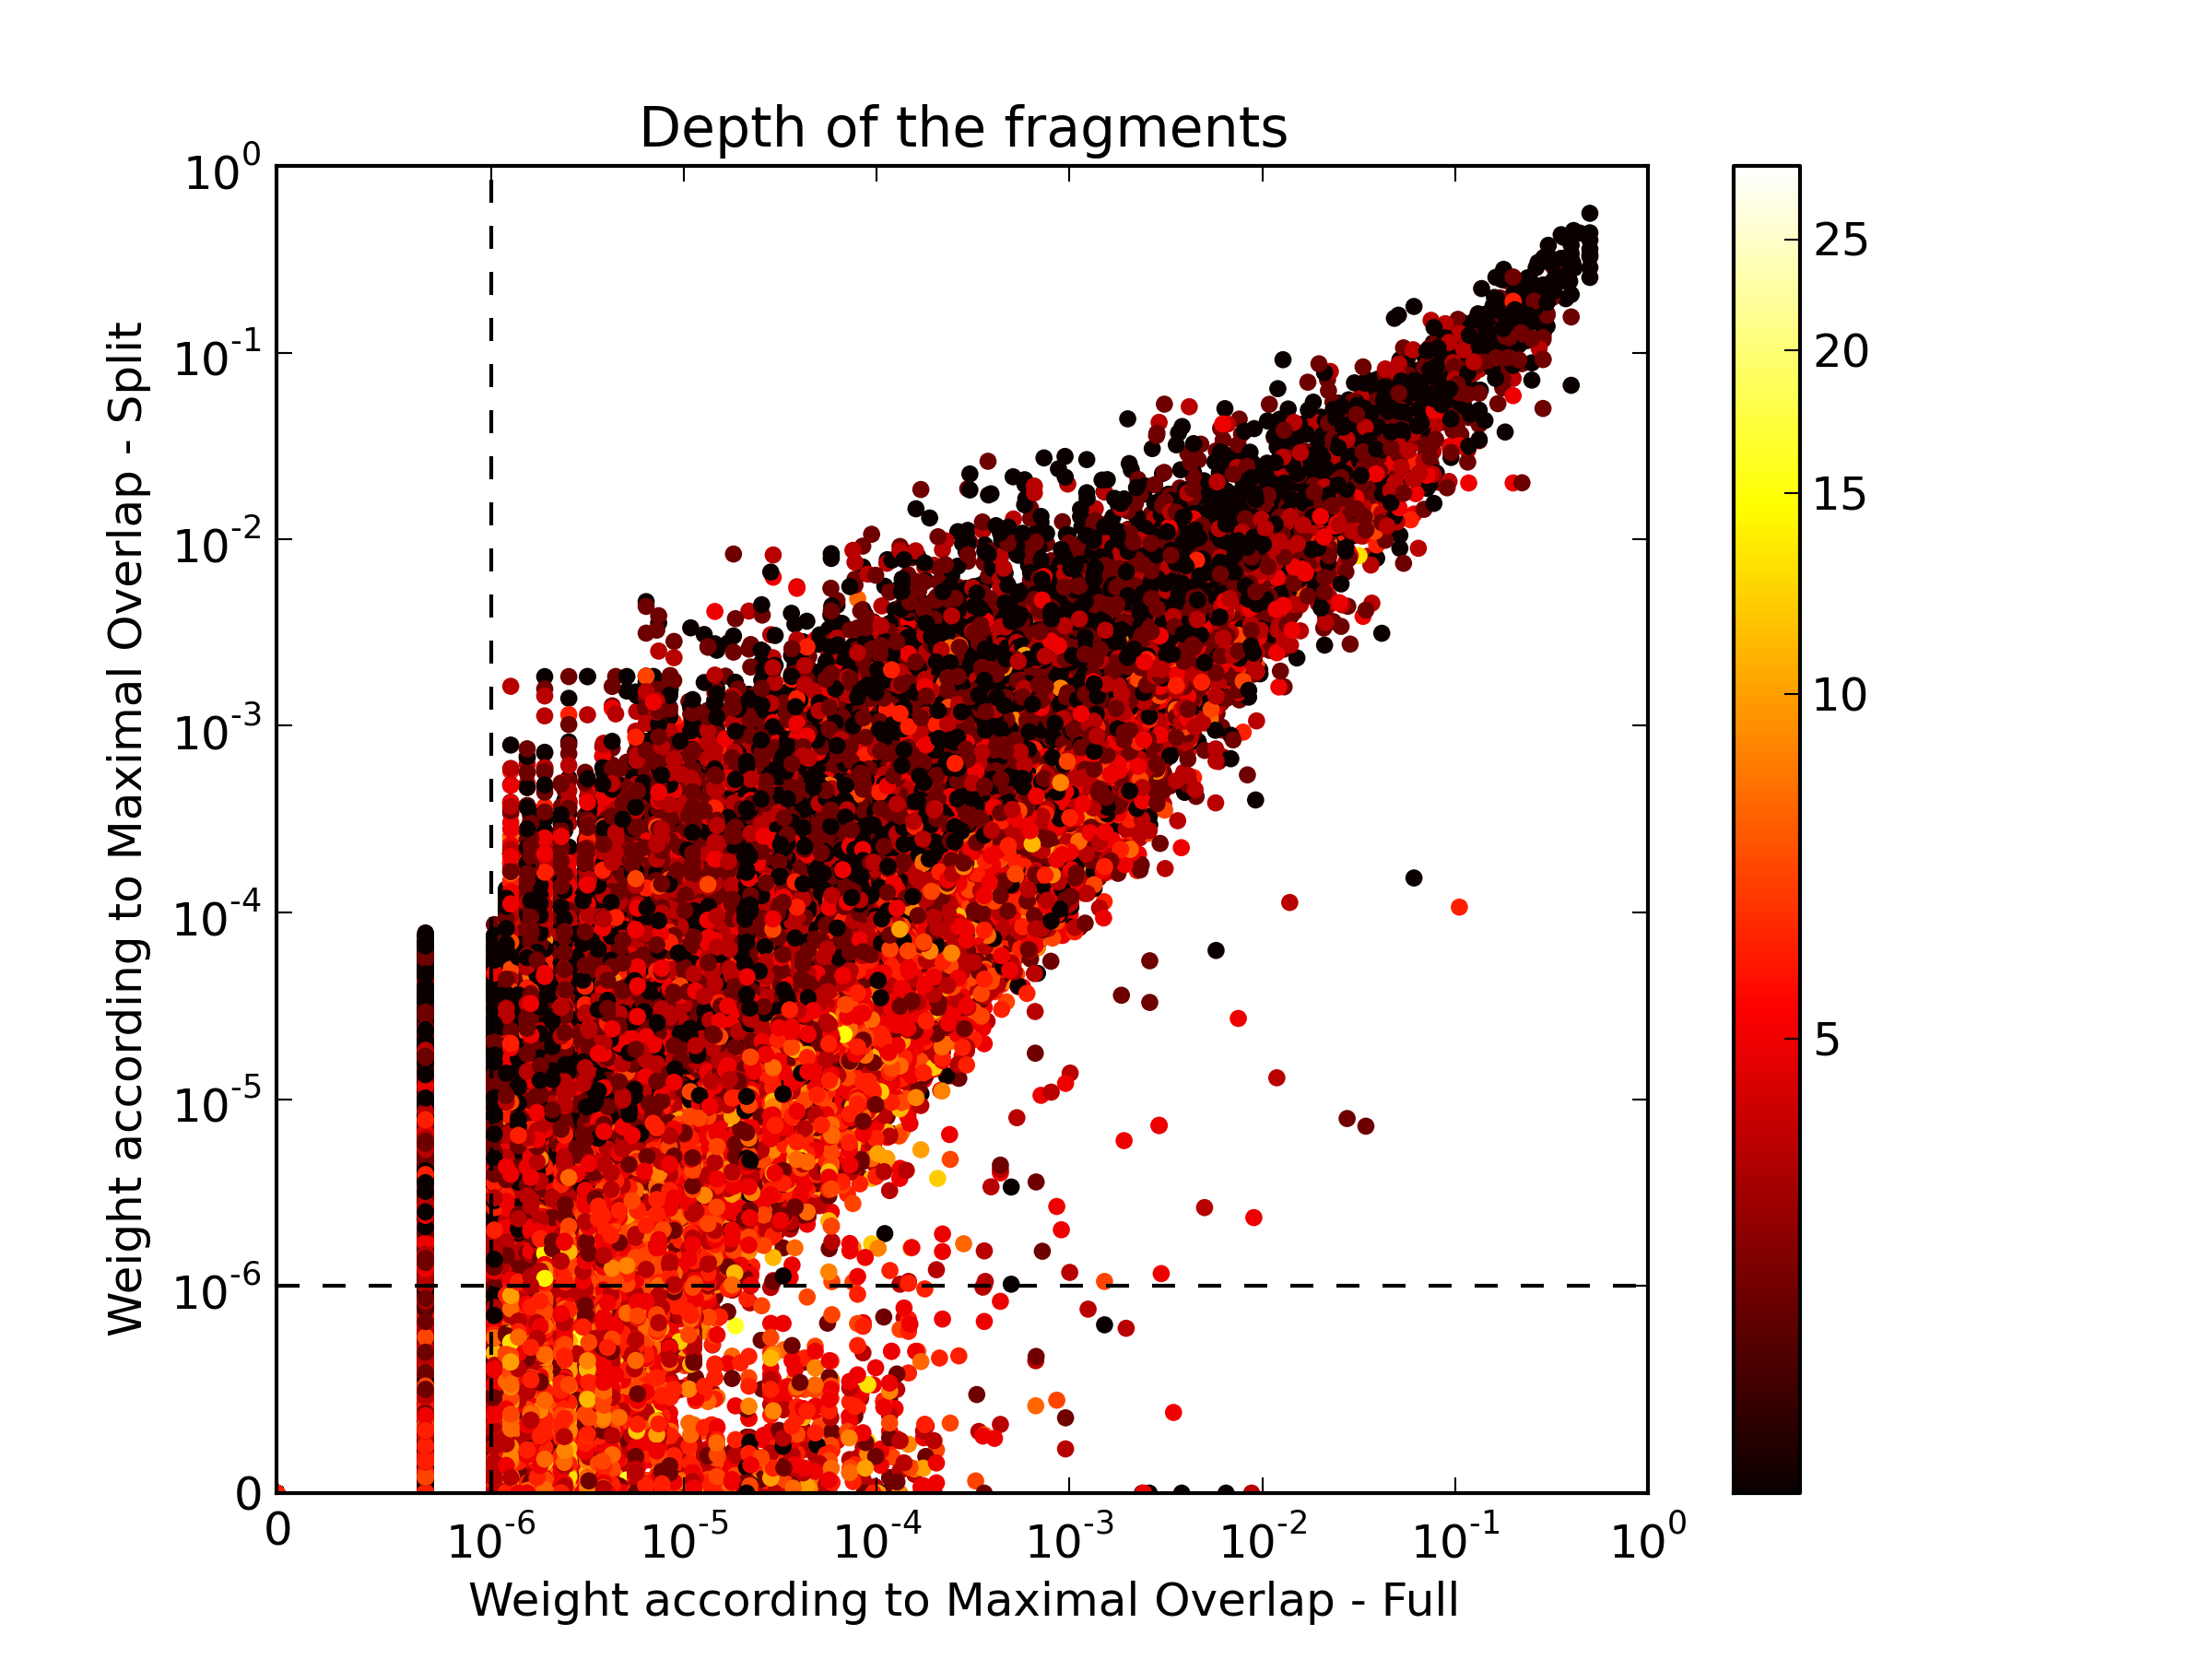
\includegraphics[width=\linewidth,trim=0.5cm 0cm 2.5cm 0.5cm, clip=true]{../data/plots/2.png}
\caption{}
\label{f:MOS-MOF}
\end{subfigure}

\caption{Comparing three grammars by depth of the fragments}
\label{f:depth3}
\end{figure*}

\paragraph{Depth of the fragments}
In figure \ref{f:depth3}, the color of the points in the scatter plot refer to the depth of the fragments. Depth is a common measure of fragment size. Johnson shows in \shortcite{johnson2002} that the original DOP1 had a bias towards larger fragments. 

Plot \ref{f:MOS-MOF} illustrates the effect of the split estimation as compared to full estimation. We see a remarkable, almost linear separation of fragments with larger depth (lighter color) below the identity line, and fragments with smaller depth above it. This indicates that the split estimation tends to reduce the bias towards larger fragments.

In plots \ref{f:SDS-MOS} and \ref{f:SDS-MOF}, the shortest derivation extraction is compared to both maximal overlap grammars. Although the correlation between weight assignment and depth is less evident, the area above the identity line gets fragments with a lighter color. This reveal that shortest derivation extraction gives a higher weight to large fragments than maximal overlap. 


\paragraph{Width of the fragments}

The width of the fragments is another measure of their size. It is defined as the number of substitution sites plus the number of terminals.As an example, in figure \ref{f:width1a} both extraction methods are compared with split estimation.  The dark peak on the right corresponds to the smoothing: PCFG fragments have low width by definition. In figure \ref{f:width1b} only fragments of depth 2 and deeper are shown, and the dark peak is gone.

The way the fragments with certain width are distributed does not differ much from the depth, of course width and depth are strongly correlated themselves. We have also looked at the number of substitution sites and the number of terminals of isolation, but this did not reveal much more than the total width. 



\begin{figure*}
\center
\begin{subfigure}{0.45\textwidth}
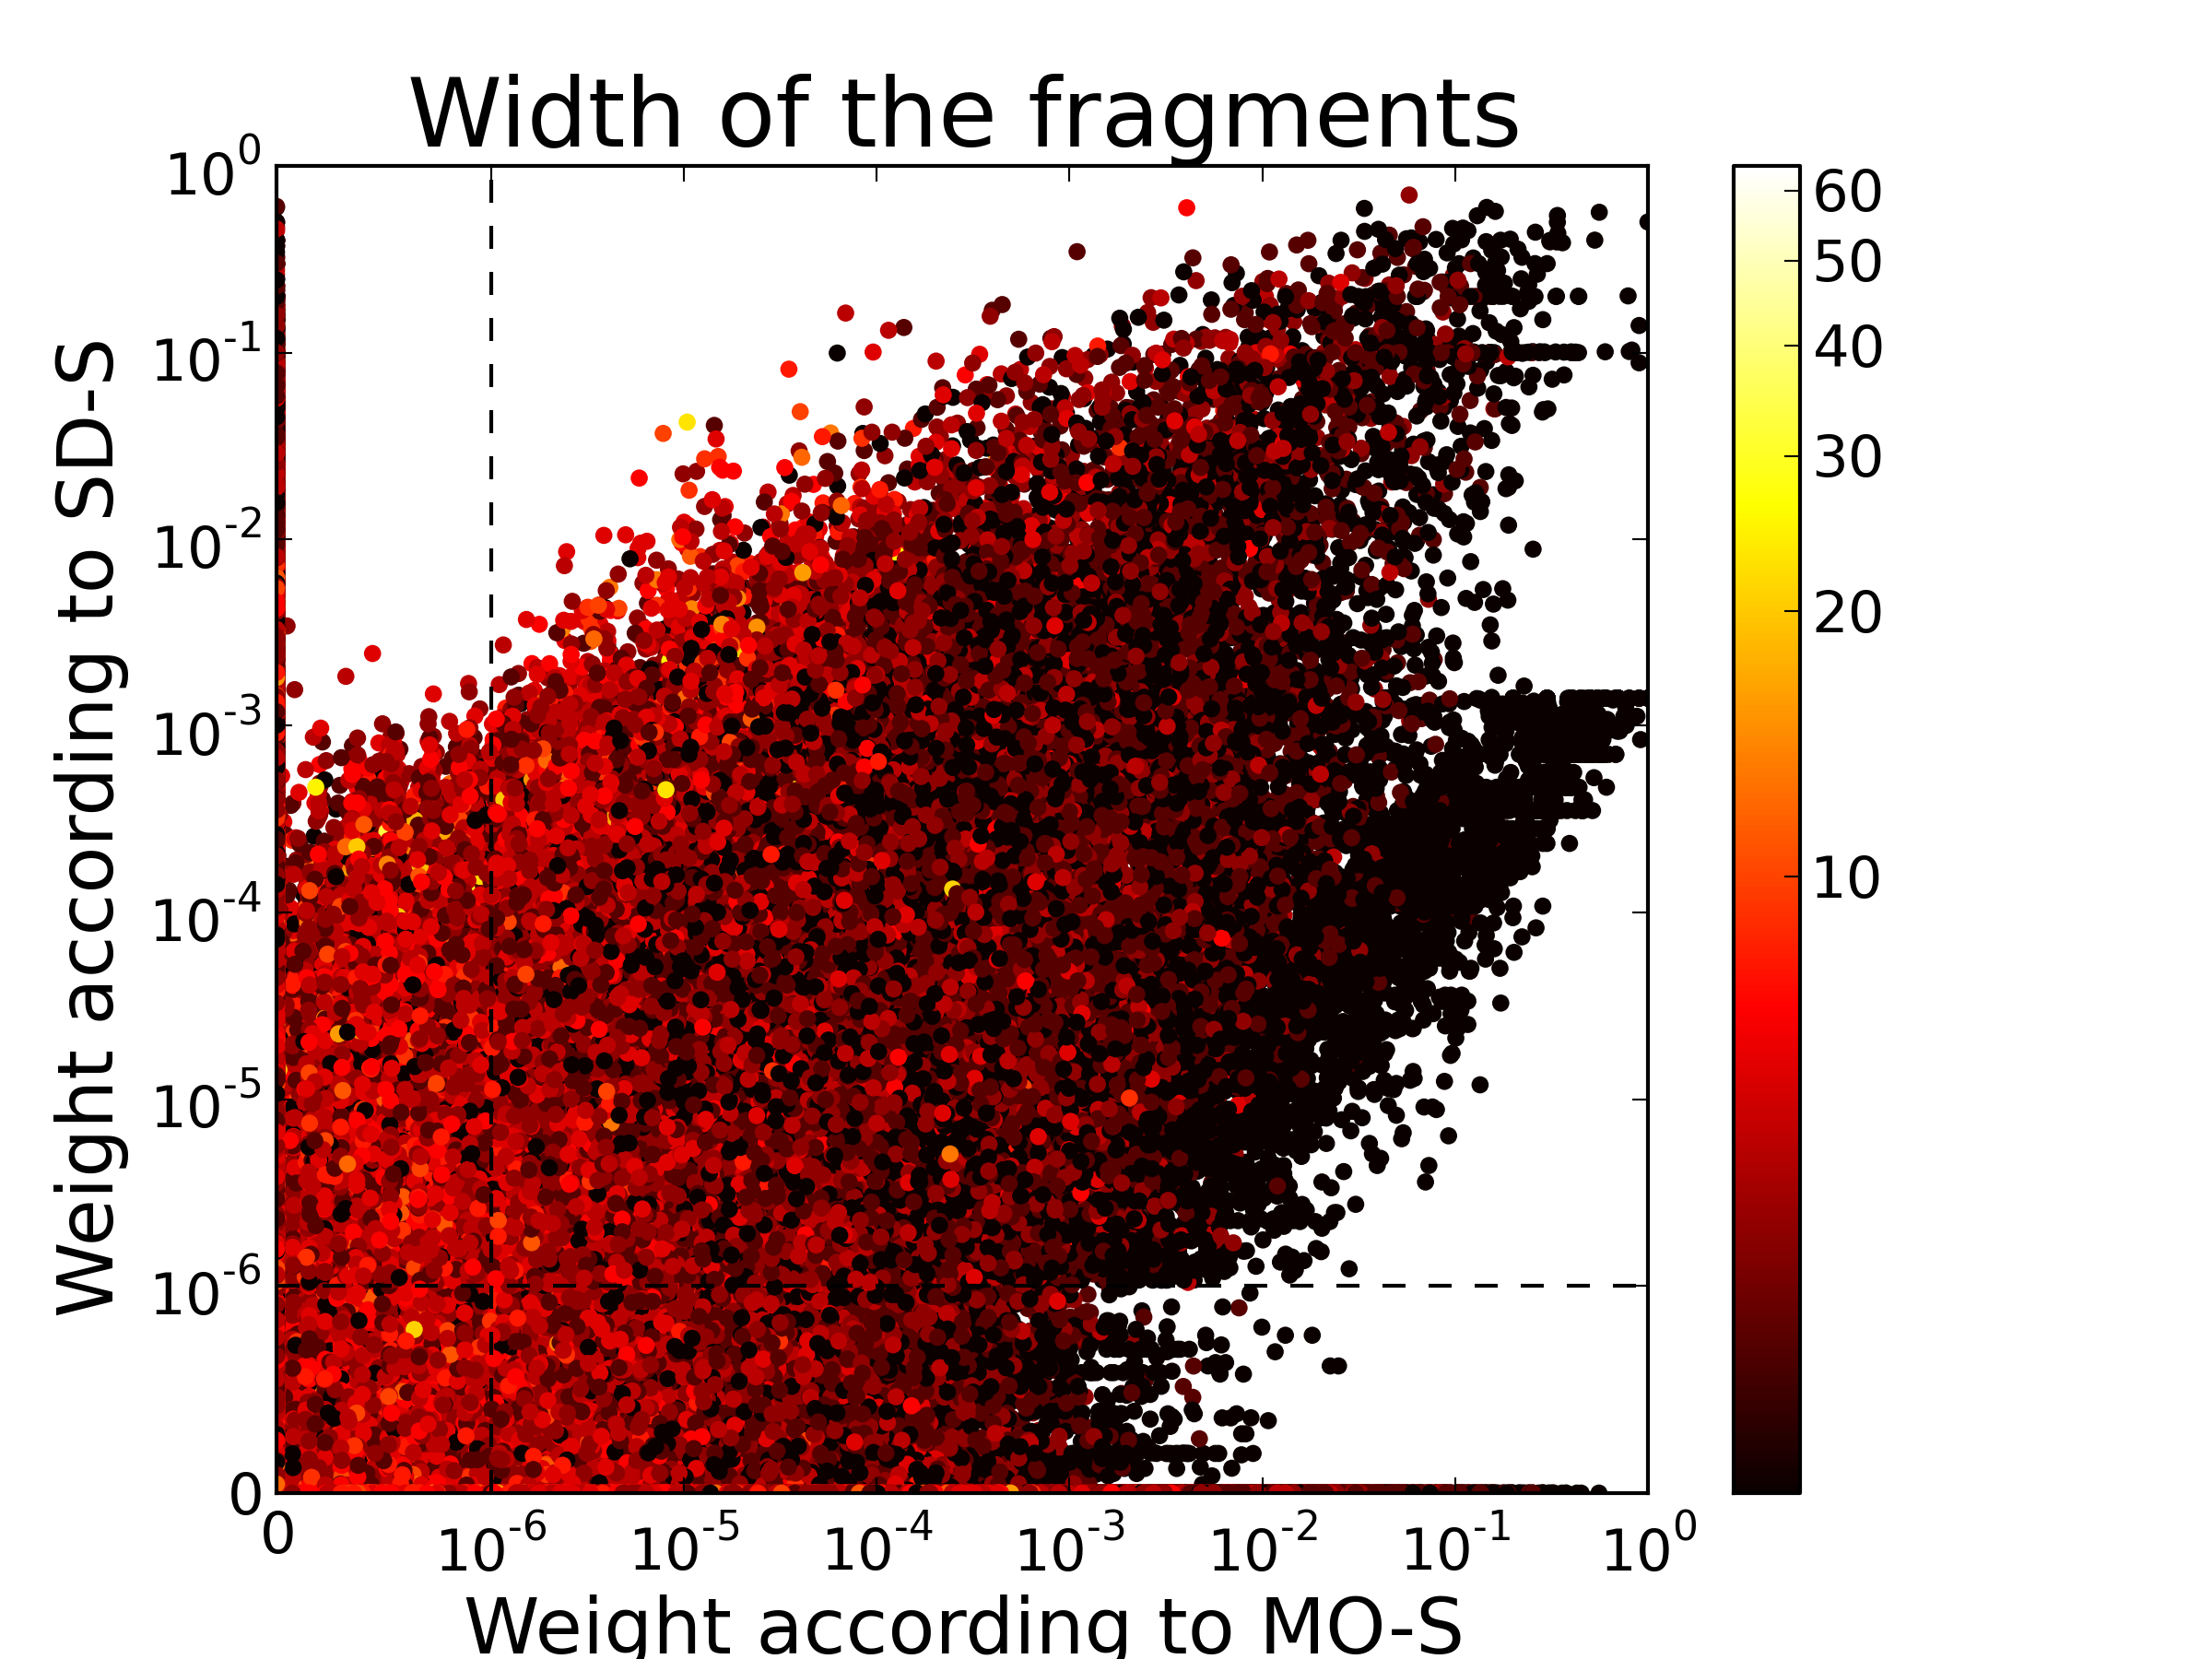
\includegraphics[width=\linewidth,trim=0.5cm 0cm 2.5cm 0.5cm, clip=true]{../data/plots/6.png}
\caption{}
\label{f:width1a}
\end{subfigure}
\begin{subfigure}{0.45\textwidth}
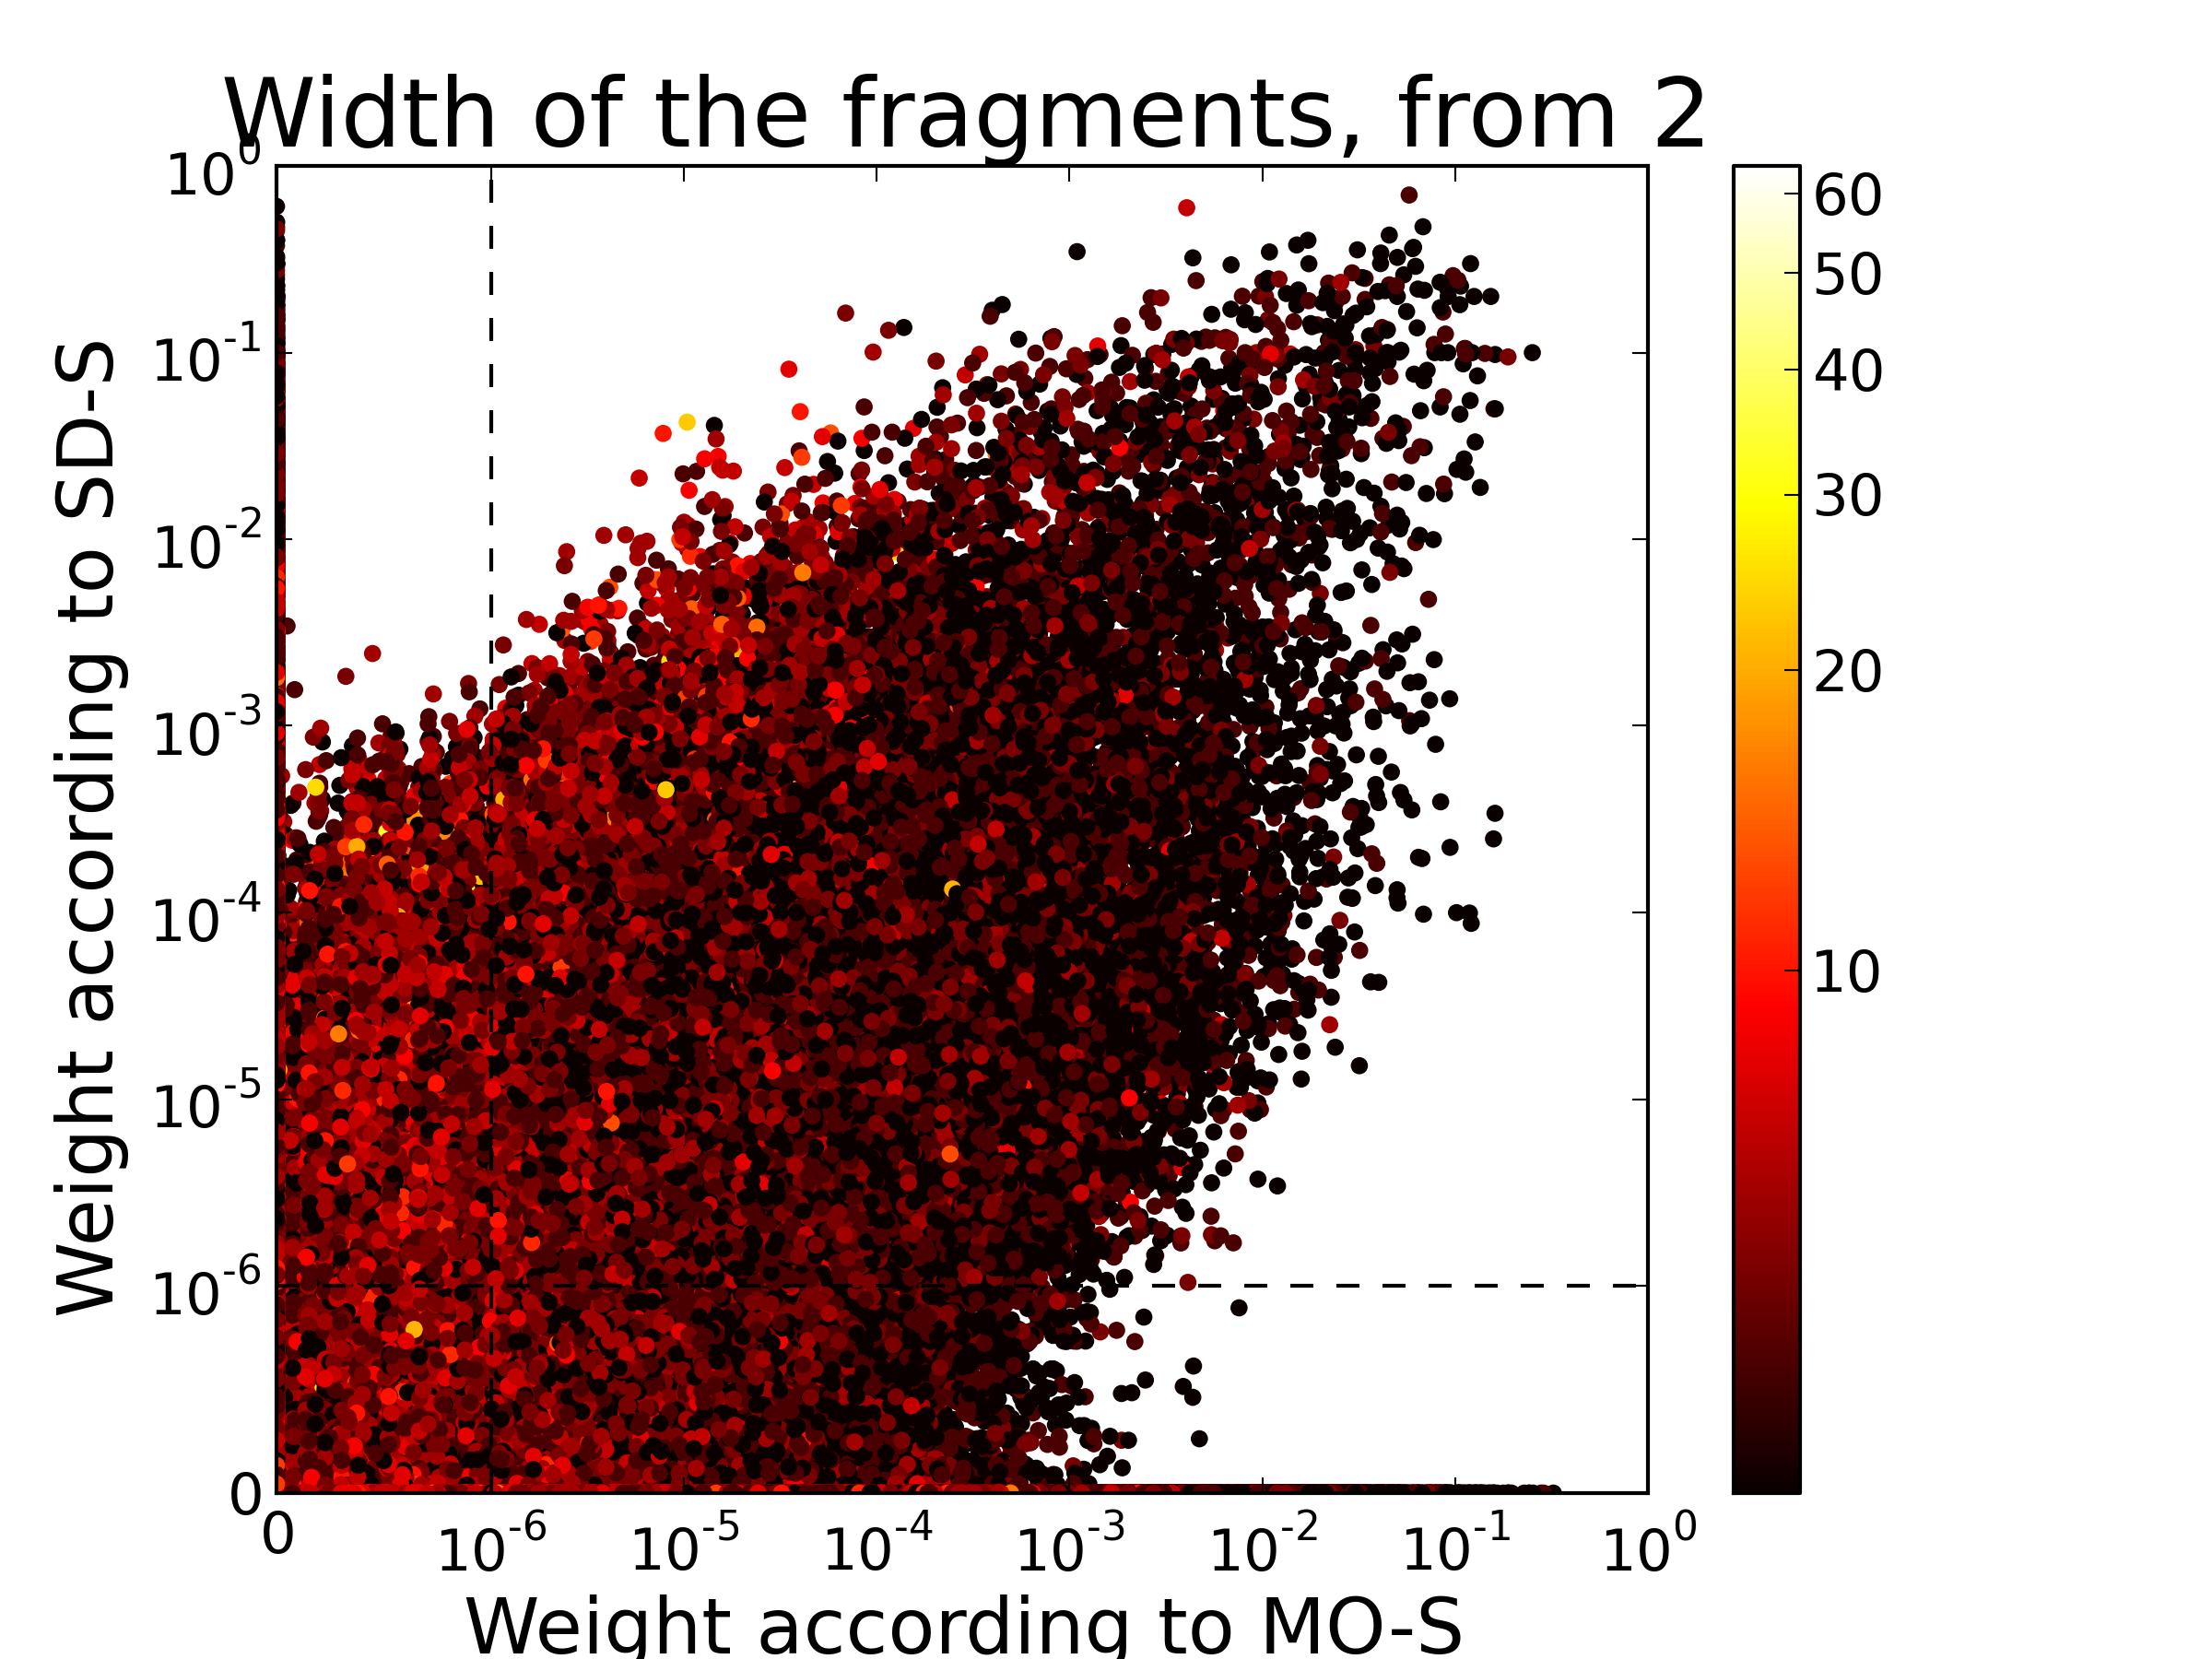
\includegraphics[width=\linewidth,trim=0.5cm 0cm 2.5cm 0.5cm, clip=true]{../data/plots/9.png}
\caption{Only fragments of depth 2 and deeper}
\label{f:width1b}
\end{subfigure}
\caption{Comparing shortest derivation to maximal overlap extraction by width of the fragments}
\label{f:width1}
\end{figure*}


%Diepe fragmenten zijn zwaarder in :
%	SD dan in MOS
%	SD dan MO
%	MO dan MOS (scherp)

%Brede fragmenten zijn zwaarder in:
% 	SD dan MOS (punt: CFG rules)
%	MO dan MOS (scherp)









%SDS MOS width



















\section{Conclusion}
%Discussion, future work

We have investigated two existing estimators in the Data Oriented Parsing approach to natural language syntax: \ddop{} and \dops. Our main question concerned the correspondence between theoretical properties and practical performance. 

%Double-DOP: best performance
%Performance not correlated with consistency of the method
%Shortest derivation, very short grammar. But not as useful as it would seem: bad performance
We compared the theoretically attractive shortest-derivation fragment extraction from \dops{} with the practical \ddop{} approach. 
We observed that the latter performed substantially better. Because the consistent grammar performed poorer, it seems that consistency might be a less interesting property in practice.

%Split (held-out est) decreases bias towards large fragments
We introduced the corpus splitting from \dops{} into the \ddop{} approach.  We have showed that the held-out estimation makes the grammar less biased towards large fragments. However, interpolating the results of random splits did not give us the expected overfitting avoidance. 

\paragraph{Concerns}
While all grammars were trained on the same data set, the grammar from the shortest derivation with split was significantly smaller than the others. This could in itself explain the lower performance of this grammar, instead of the estimation method, because larger tree substitution grammars simply describe more data. It is therefore impossible to be completely certain in blaming the lower performance on the shortest-derivation approach. Other factors that might play a role are the usage of relative frequency (other estimates could be applied) and the smoothing method: the PCFG rules got heigher weight assignment in the \ddop{} approach. 


\paragraph{Future work}
% analysis of other DOP grammars,
Our analysis concerned only two existing DOP estimators: \ddop{} and \dops{}. Others have been proposed with one or more of the same desirable properties or comparable performance, of which the comparative analysis is future work.

%more elaborate analysis: possibly clustering on features such as depth, number of substitution sites and terminals
Additionally, the fragment weight comparision in this paper is exploratory and rough. It would be very interesting to perform clustering on features such as depth, number of substitution sites and terminals to build a model of the difference in weight distribution.

% is consistency indeed a valuable property at all?
Finally, it is an important question whether estimator consistency for DOP is a valuable property at all. Behaviour of an estimator in the limit, on finite languages and on artificial constructions is not guaranteed to lead to improved performance on real treebanks. 

\paragraph{Acknowledgements}
We would like to thank Andreas van Cranenburgh for his generous contributions to both the theoretical insights and practical implementations in this work. Without him, this work would not have been.




%\bibliographystyle{ieeetr}
%\bibliography{bibliography}

\bibliographystyle{acl2014}
\bibliography{bibliography}

\end{document}
